%% This is a simple LaTeX template for a B1 mini-project. Please send corrections to thomas.adcock@eng.ox.ac.uk

%% Last update 24/4/2020

\documentclass[11pt]{article}
%\usepackage{fontspec}
\usepackage{graphicx}
\usepackage{parskip}
\usepackage{multicol}
\usepackage{titlesec}
\usepackage{setspace}
\usepackage{amsmath}
\usepackage[margin=20 mm]{geometry}
\usepackage{hyperref}
\doublespacing
% There is some scope for changing the paragraph spacing and spacing around section headers if you are short of space

% Use Arial
%\setmainfont[
%BoldFont=Arial Bold.ttf,
%ItalicFont=Arial Italic.ttf,
%BoldItalicFont=Arial Bold Italic.ttf
%]{Arial.ttf}


\begin{document}

%% Cover page for a B1 project. This should not contain your name or college!
\begin{center}
\vspace*{2cm}
Trinity Term 2020\\ % enter the date
\vspace*{6cm}
 \huge{\textbf{{}3YP Project}}\\ 
\vspace*{6cm}
{\large{My candidate number}} % Not your Bod card number
\thispagestyle{empty} % Remove page number


\end{center}

\newpage
% You do not need a contents page in such a short report. Nor do you need a list of figures etc. However, if you think this is necessary you can uncomment the following
%\tableofcontents
%\thispagestyle{empty} % Remove page number
%\newpage

\setcounter{page}{1}

\section{Introduction}
Testing to see if commits using overleaf (paid account) works - Josh.

SMALL CHANGE

Final Test - using Latex on computer again - will this cause issues? Will make it so that commits are correctly labelled.




\section{Tables}

\LaTeX{} produces neat tables although they can be slightly fiddly to create. There are tools for copying tables from Excel. Table \ref{tab:latesubpen} is an example table. Tables should be referenced in the text before they appear on the page and have a caption which explains what is in the table.
\begin{table}[h] % the [h] forces the table to be "here". This is quite a short document so LaTeX struggles to find a nice arrangement for the floats! Not normally needed
\begin{center}
\begin{tabular}{ |l|c| } 
 \hline
  Time after deadline & Penalty  \\ 
  \hline
 4 hours & 1\%  \\ 
 1 day & 10\%  \\ 
 2 days & 20\%  \\ 
 5 days & 50\%\\
 \hline
\end{tabular}
\end{center}
\label{tab:latesubpen}
\caption{Standard penalties for late submission of B1 project.}
\end{table}



\section{Figures}

Figure \ref{fig:examplebargraph} is an example figure. Figures should be referred to in the text before they appear on the page and should have a caption explaining the figure. No figure should appear without being referred to. Vector graphics should be used for figures to avoid  pixelated images. When outputting from MATLAB .pdf is best although .eps and other formats can also be used. The only exception to the vector graphics rule is where surf plots (or similar) are used.

\begin{figure}
\centering
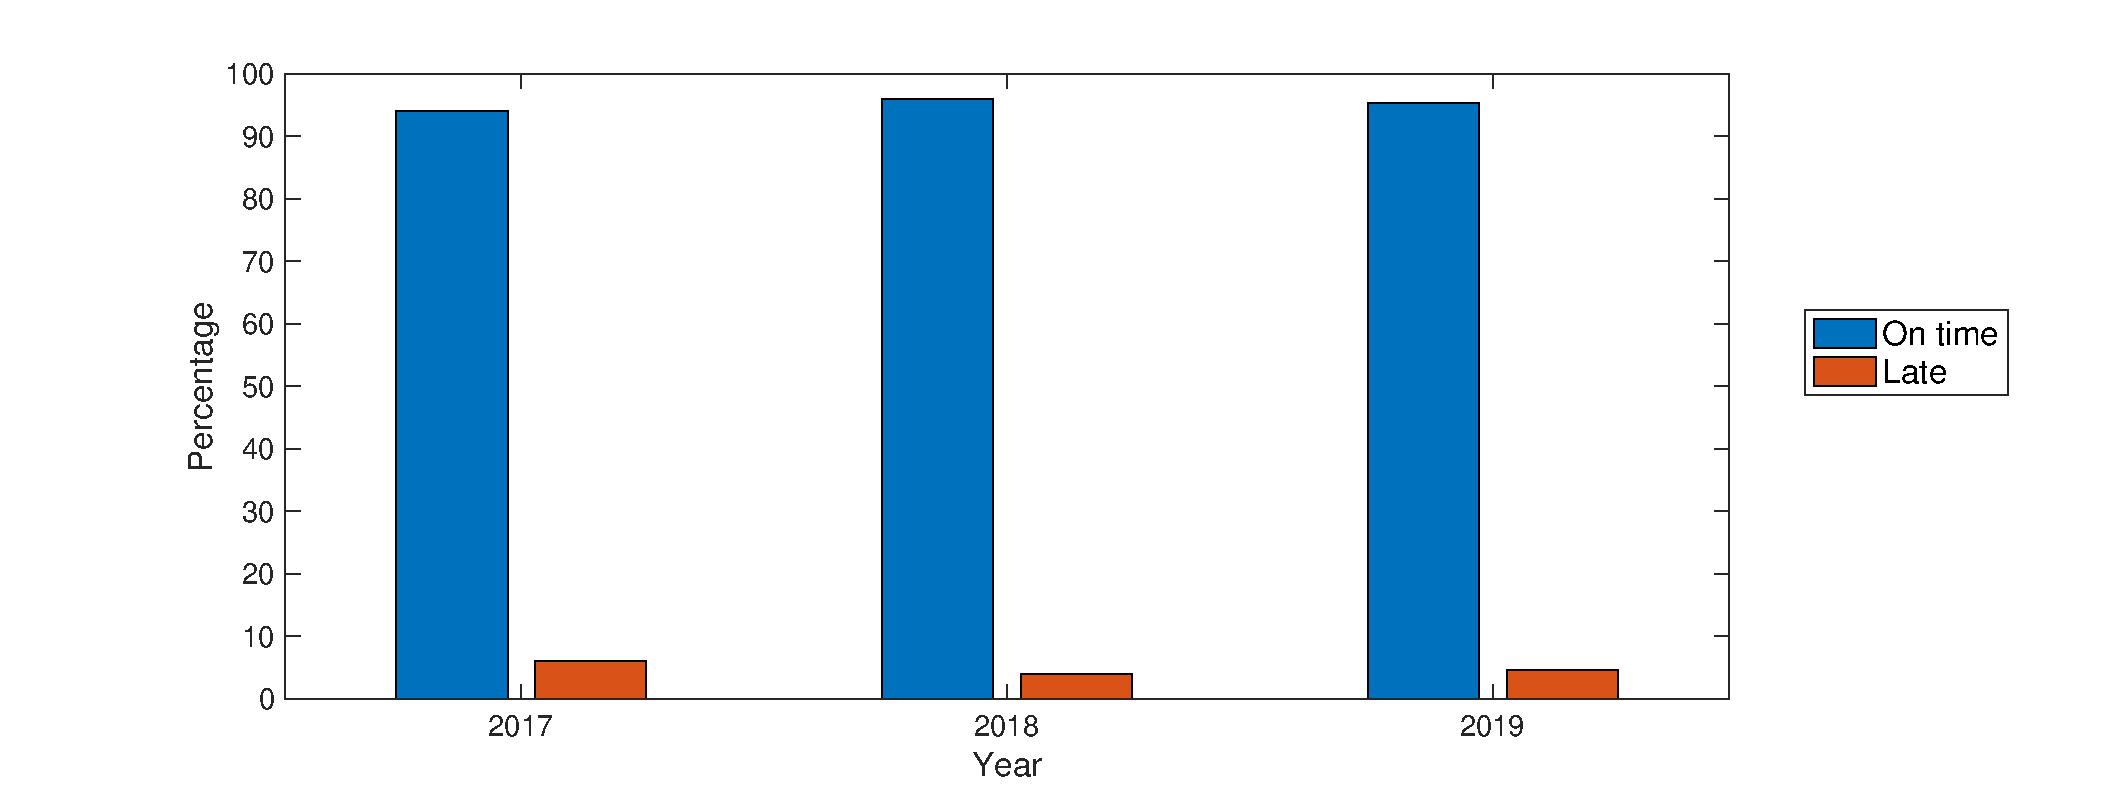
\includegraphics[width=0.8\textwidth]{asimplebarchart.eps}
\caption{Number of students submitting their B1 project on time or late over several years (approximate data).}
\label{fig:examplebargraph}
\end{figure}

\section{Quoting code}
The verbatim environment should be used if you put code in your report.
\begin{verbatim}
10 PRINT "HELLO WORLD ";
20 GOTO 10
\end{verbatim}
Most students put in too much code. Code should only be included if it is the best way of communicating how an algorithm works. Usually words or even a flow chart do this more effectively.

\section{Equations}
The are two basic ways to do equations in \LaTeX. They can be `inline' such as $y=A\cos\left(\pi x\right)$. Alternative they can be be `displayed'. An example of this would be:
\begin{equation}
    E=mc^2,
    \label{eq:Einstien}
\end{equation}
where $E$ is energy, $m$ is mass and $c$ is the speed of light.

Or you can do several equations together.
\begin{align}
    v&=u+a t,\label{eq:SUVAT1}\\
    v^2&=u^2+2 a s,\\
    s&=ut+\frac{1}{2}at^2.\label{eq:SUVAT3}
\end{align}
Note that, in general, variables in equation must be defined in the text as was done for Equation \ref{eq:Einstien}. In the B1 projects are to some extent an exception to this. In these variables defined in the project brief can be used without definition in your report.



\section{Citations}

In general we are happy if references use a smaller font and line-spacing than the rest of the text. However, do not go too far--they must still be easy to read.

Referencing may be done using any sensible method. Typically either `Harvard' referencing (name (date)) or numbered referencing will be used\footnote{Humanities students use footnotes for referencing. We do not generally use this form in engineering.}. You can choose. It is easy to switch between different referencing styles by changing the bibliographystyle at the end of this file. Try different ones and see which you prefer. Note in most technical documents the list of citations should have the title `References' and not `Bibliography' which is a slightly different thing.

This document uses bibtex for managing references. If you want to cite something you need to create an entry in a bibtex file (in this case mybib.bib). For items in the published literature use Google Scholar to search for them and then export the citation in bibtex format (note this is buggy and you often have to edit this). Some examples are  \cite{WilliamsTodd,coussios2008applications,mei2009constant} as well as the thesis of the most famous graduate of the department \cite{RowanAtkinsonthesis}. 


\begingroup\onehalfspacing
{\small
%\renewcommand{\section}[2]{}
\begin{multicols}{2}
\bibliographystyle{unsrt}
%\bibliographystyle{elsarticle-num}
% \bibliographystyle{elsarticle-harv}
% \bibliographystyle{elsarticle-num-names}
% \bibliographystyle{model1a-num-names}
% \bibliographystyle{model1b-num-names}
% \bibliographystyle{model1c-num-names}
% \bibliographystyle{model1-num-names}
% \bibliographystyle{model2-names}
% \bibliographystyle{model3a-num-names}
% \bibliographystyle{model3-num-names}
% \bibliographystyle{model4-names}
% \bibliographystyle{model5-names}
% \bibliographystyle{model6-num-names}
\bibliography{mybib}
\end{multicols}}
\endgroup
\end{document}
